\documentclass[a4paper,12pt]{article} % тип документа

%  Русский язык
\usepackage[T2A]{fontenc}			  % кодировка
\usepackage[utf8]{inputenc}			  % кодировка исходного текста
\usepackage[english,russian]{babel}	  % локализация и переносы
\usepackage{graphicx}                 % импорт изображений

% Математика
\usepackage{amsmath,amsfonts,amssymb,amsthm,mathtools} 

% Другие пакеты
\graphicspath{{images/}{images2/}}    % папки с картинками
\usepackage{hyperref}                 % ссылки на странцы

\usepackage{caption}
\captionsetup{justification=centering}

% вид страницы
\usepackage{geometry} % Простой способ задавать поля
	\geometry{top=25mm}
	\geometry{bottom=35mm}
	\geometry{left=35mm}
	\geometry{right=20mm}

% ==================================================================================================

\begin{document}
    % ==================================================================================================
    \begin{center}
        \normalsize{МИНИСТЕРСТВО ОБРАЗОВАНИЯ И НАУКИ РОССИЙСКОЙ ФЕДЕРАЦИИ\\ 
                    МОСКОВСКИЙ ФИЗИКО-ТЕХНИЧЕСКИЙ ИНСТИТУТ \\ 
                    (ГОСУДАРСТВЕННЫЙ УНИВЕРСИТЕТ)\\
                    ФИЗТЕХ-ШКОЛА АЭРОКОСМИЧЕСКИХ ТЕХНОЛОГИЙ\\
                    КАФЕДРА ПРИКЛАДНОЙ МЕХАНИКИ}
        
        \vspace{13ex}
        
        \normalsize{Лабораторная работа №1\\}
        \vspace{5ex}
        \textbf{Обработка показаний Фурье-спектрометра.}

        \vspace{15ex}

        \normalsize{Выполнил:\\
                    студент группы Б0Х-ХХХ\\
                    Имя Фамилия}
        
    \end{center}
            
    \vfill
            
    \begin{center}
        г. Долгопрудный\\ 
        2021 г.
    \end{center}

    \thispagestyle{empty} % выключаем отображение номера для этой страницы
    \newpage
    % ==================================================================================================

    % --------------------------------------------------------------------------------------------------
    \tableofcontents{} %содержание
    \newpage
    % --------------------------------------------------------------------------------------------------

    \section{Принцип работы}

    % Вопрос: как сделать, чтобы после \section была красная строка?
    % Ответ: этого делать не надо, \LaTeXL лучше знает, как будет красиво. 
    % Если таковы требования по оформлению документа, можно подключить пакет \usepackage{indentfirst}. 
    % Однако выглядеть это будет омерзительно. Если делать смещение первой строке, то делать его и заголовку.

    Фурье-спектрометр -- оптический прибор, используемый для количественного и качественного анализа содержания веществ в газовой пробе. 
    Основным элементом оптической схемы Фурье-спектрометра является двухлучевой интерферометр Майкельсона, 
    состоящий из полупрозрачного светоделителя и двух плоских зеркал. 
    Фурье-спектрометр позволяет получать информацию о спектральном составе ИК излучения и, следовательно, 
    об электромагнитных свойствах исследуемых объектов в окрестности длин волн 1 -- 10 мкм. 
    Схема устройства Фурье-интерферометра представлена на рисунке \hyperref[picture_1]{1}.

    \begin{figure}[h!]
        \centering
        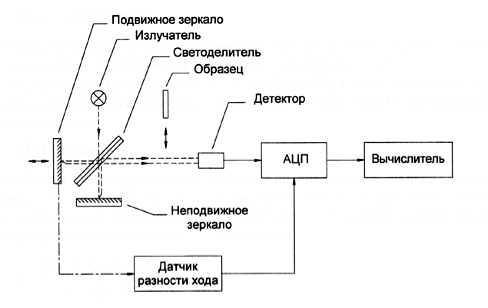
\includegraphics[width=0.48\linewidth]{1.png}
        \label{picture_1}
        \caption{Схема устройства Фурье-интерферометра}
    \end{figure}

    Излучение от излучателя падает на полупрозрачную поверхность светоделителя и расщепляется на два пучка. 
    После отражения от соответствующих зеркал интерферометра излучение двух пучков складывается на светоделителе и направляется на детектор, 
    преобразующий его в электрический сигнал. Если одно из зеркал двухлучевого интерферометра Майкельсона перемещать, 
    то оптический путь для соответствующего пучка будет изменяться, 
    и в точке приема интенсивность излучения будет меняться вследствие интерференции волн двух пучков, 
    отражающихся от подвижного и неподвижного зеркал.

    Зависимость регистрируемого сигнала от оптической разности хода пучков называется интерферограммой. 
    Максимум сигнала интерферограммы соответствует нулевой разности хода, 
    так как в этом случае все спектральные составляющие излучения пучков приходят в точку приема в фазе. 
    Интерферограмма содержит информацию о спектральном составе излучения. 
    Однако получить данную информацию в явном виде можно только после применения преобразования Фурье.

    \newpage

    \section{Измерения}

    В ходе лабораторной работы было получено три интерферограммы: 
    для пустого канала, канала со стеклом и канала со стеклом, покрытым CuO. 
    Соответствующие интерферограммы изображены на рисунках \hyperref[picture_2]{2}, \hyperref[picture_3]{3}, \hyperref[picture_4]{4}.

    \begin{figure}[h!]
        \begin{center}
            \begin{minipage}[h!]{0.4\linewidth}
                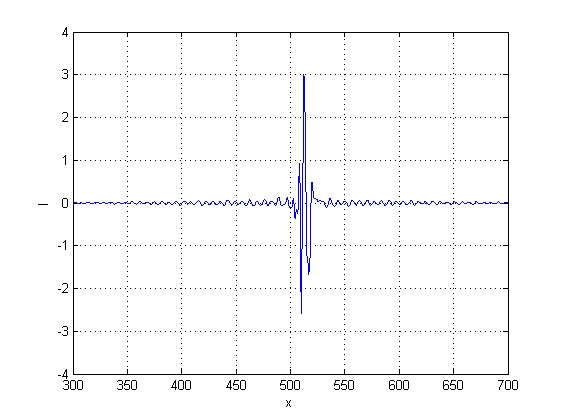
\includegraphics[width=1.2\linewidth]{2.png}
                \caption{Экспериментально полученная интерферограмма для пустого канала}
                \label{picture_2}
            \end{minipage}
            \hfill
            \begin{minipage}[h!]{0.4\linewidth}
                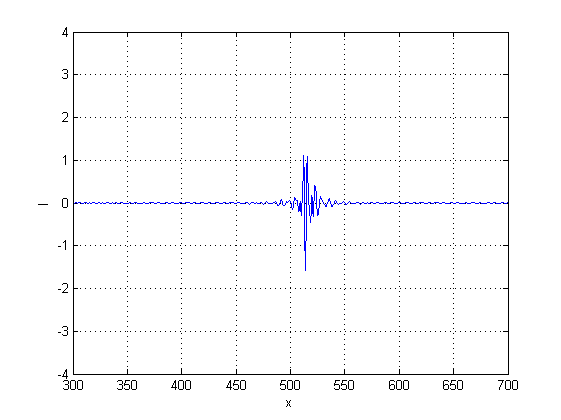
\includegraphics[width=1.2\linewidth]{3.png}
                \caption{Экспериментально полученная интерферограмма для стекла}
                \label{picture_3}
            \end{minipage}
        \end{center}
    \end{figure}

    %! какие-то проблемы с подписью к 4му рисунку. Почему-то она не центрируется. Исправить.

    \begin{figure}[h!]
        \centering
        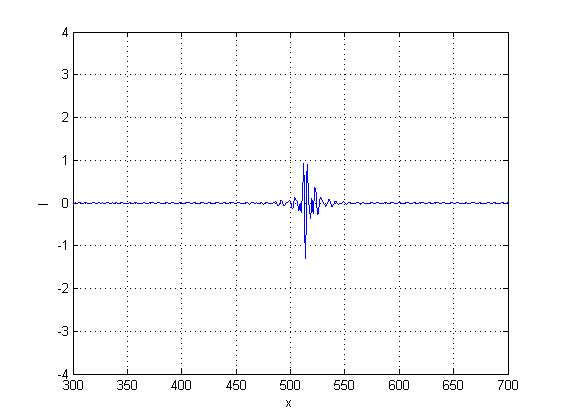
\includegraphics[width=0.48\linewidth]{4.png}
        \label{picture_4}
        \caption{Экспериментально полученная интерферограмма для стекла с напылением CuO}
    \end{figure}

    Однако, из рисунков совершенно неочевидны электромагнитные свойства исследуемых образцов, 
    поскольку они представляют собой лишь зависимость интенсивности излучения в точке приёма. 
    Для удобства восприятия прибор сдвигает графики по оси  на величину . 
    Таким образом, зависимости, представленные на графиках представляются формулой \eqref{formula_1}:

    \begin{equation} \label{formula_1}
        \Delta I = I(x) - I(0)
    \end{equation}

    Преобразование Фурье в данном случае будет описываться следующим образом:

    \begin{equation}
        S(k) = \int^{x_{max}}_{0} [I(x) - I(0)] e^{i 2 \pi kx} dx
    \end{equation}

    где – максимальная оптическая разность хода, k – волновое число, равное:

    \begin{equation}
        k = \frac{10^{-4} \text{[мкм/см]}}{\lambda \text{[мкм]}}
    \end{equation}

    \section{Расчеты в MATLAB}

    Над полученными интерферограммами в среде MATLAB было произведено дискретное преобразование Фурье. 
    Соответствующие коэффициенты разложения по волновым числам представлены на рисунках 
    \hyperref[picture_5]{5}, \hyperref[picture_6]{6}, \hyperref[picture_7]{7}, \hyperref[picture_8]{8}.

    \begin{figure}[h!]
        \begin{center}
            \begin{minipage}[h!]{0.4\linewidth}
                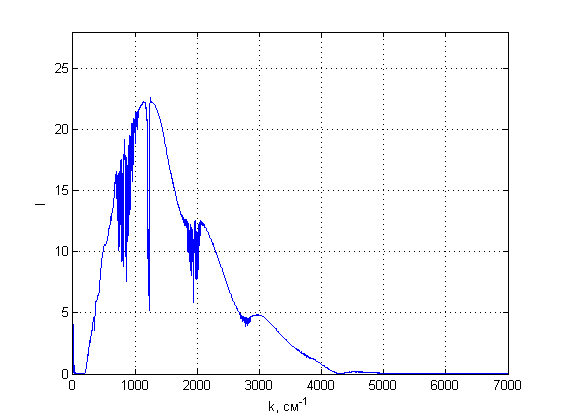
\includegraphics[width=1.2\linewidth]{5.png}
                \caption{ПФ интерферограммы для пустого канала}
                \label{picture_5}
            \end{minipage}
            \hfill
            \begin{minipage}[h!]{0.4\linewidth}
                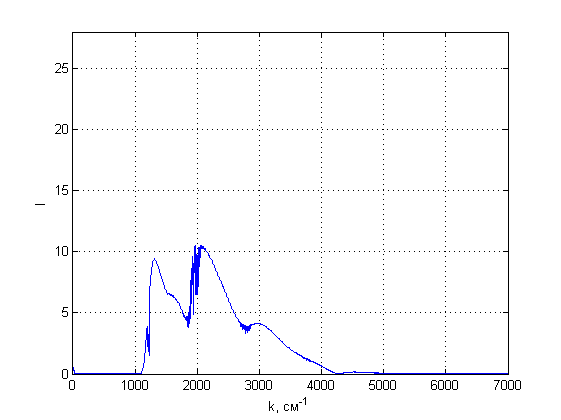
\includegraphics[width=1.2\linewidth]{6.png}
                \caption{ПФ интерферограммы для стекла}
                \label{picture_6}
            \end{minipage}
            \hfill
            \begin{minipage}[h!]{0.4\linewidth}
                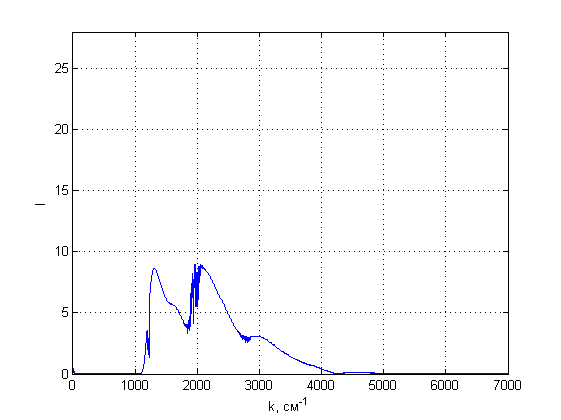
\includegraphics[width=1.2\linewidth]{7.png}
                \caption{ПФ интерферограммы для стекла с напылением CuO}
                \label{picture_7}
            \end{minipage}
            \hfill
            \begin{minipage}[h!]{0.4\linewidth}
                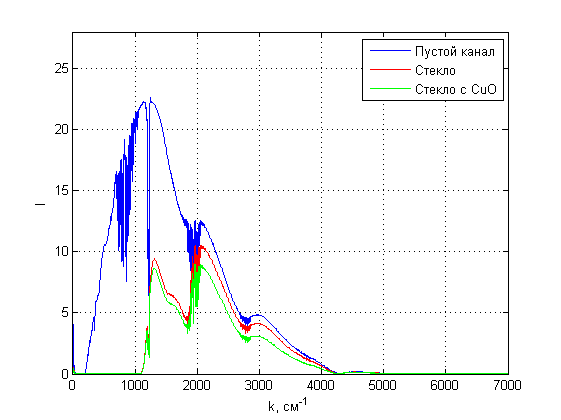
\includegraphics[width=1.2\linewidth]{8.png}
                \caption{Сводный график}
                \label{picture_8}
            \end{minipage}
        \end{center}
    \end{figure}

    Для получения спектра пропускания материалов было найдено отношение спектральной плотности прошедшего через образец сигнала 
    к спектральной плотности сигнала, прошедшего через пустой канал. Графики отношений представлены на рисунках 
    \hyperref[picture_9]{9}, \hyperref[picture_10]{10}.

    \newpage

    \begin{figure}[h!]
        \begin{center}
            \begin{minipage}[h!]{0.4\linewidth}
                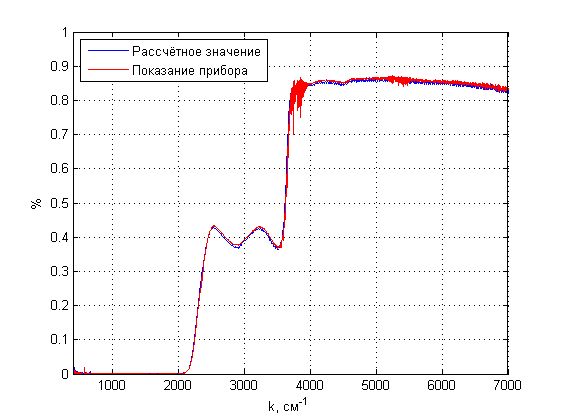
\includegraphics[width=1.2\linewidth]{9.png}
                \caption{Коэффициент пропускания стекла}
                \label{picture_9}
            \end{minipage}
            \hfill
            \begin{minipage}[h!]{0.4\linewidth}
                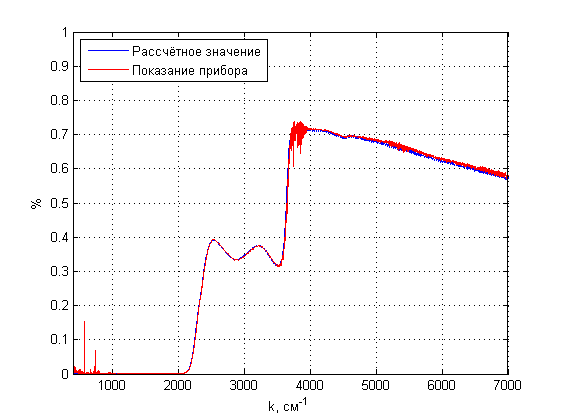
\includegraphics[width=1.2\linewidth]{10.png}
                \caption{Коэффициент пропускания стекла с напылением CuO}
                \label{picture_10}
            \end{minipage}
        \end{center}
    \end{figure}

\end{document}